\documentclass{beamer}
\usetheme{AnnArbor}
\usepackage{graphicx}
\graphicspath{{pics/}}
\usepackage{amsmath}
\usepackage{amssymb}
\usepackage{framed}
\usepackage{tikz}
\usepackage[]{xcolor}
\usepackage[most]{tcolorbox}
\usepackage{pgfplots}
\pgfplotsset{compat=1.18}
\usepackage{blkarray}
\setbeamercolor{mycolorbox}{%
  bg=yellow!20,   % background color (20% yellow)
  fg=black      % foreground (text) color
}
\usefonttheme[onlymath]{serif}

\newtcolorbox{solutionblock}{
  colback=yellow!5,        % Background color: light yellow
  colframe=orange!80!black, % Frame color: dark orange
  title=Solution,
  fonttitle=\bfseries
}

\title{Linear,Quadratic, Polynomial and Rational Functions}
\author{Nithin}
\institute{}
\date{\today}
\begin{document}
\begin{frame}
  \titlepage
\end{frame}
\begin{frame}
  \tableofcontents
\end{frame}

  \subsection{Lines and Linear Function}
  \begin{frame}{Slope}
    \begin{figure}
      \centering
      \includegraphics[scale=0.25]{slope.png}
    \end{figure}

    \[\frac{y_{2} - y_{1}}{x_{2} - x_{1}} = \frac{y_{4} - y_{3}}{x_{4} - x_{3}}\]
  \end{frame}
  \begin{frame}
    \frametitle{Slope}
    \begin{block}{Definition}
      If \(x_{1},y_{1}\) and \(x_{2},y_{2}\) are any two points on a line with \(x_{1} \neq x_{2}\), then the \textbf{slope}
      of the line is 
      \[\frac{y_{2} - y_{1}}{x_{2} - x_{1}}\] 
    \end{block}
  \end{frame}

  \begin{frame}
    \frametitle{Slope}
    
    \begin{columns} 
      \column{0.5\textwidth} 
      \textbf{Key Points:}
      \begin{itemize}
          \item Positive slope slands up from left to right 
          \item Negative slope slands down from left to right 
          \item Horizontal line has slope = 0
          \item Vertical line has no slope
      \end{itemize}
  
      \column{0.5\textwidth} % Right column - 50% width
      \centering
      \includegraphics[width=0.8\linewidth]{slope2.png} % Replace with your image filename
  \end{columns}
  \end{frame}

\begin{frame}
  \frametitle{Line Equation}
  \begin{columns} 
    \column{0.5\textwidth} 
  \begin{alertblock}{slope and one point on it}
    The line in the xy-plane that has slope \(m\) and contains the point \((x1, y1)\) is given
by the equation 
\[y - y_{1} = m(x  -  x_{1})\]
  \end{alertblock}

  \column{0.5\textwidth} % Right column - 50% width
  \centering
  \includegraphics[width=0.8\linewidth]{line1.png} % Replace with your image filename
  \end{columns}

\end{frame}

\begin{frame}
  \frametitle{Line Equation}
  \begin{columns} 
    \column{0.5\textwidth} 
  \begin{alertblock}{slope and \(y\) intercept}
    The line in the xy-plane with slope \(m\) that intersects the \(y\) axis at \(0,b\) is given by the equation 
by the equation 
\[y = mx+b\]
  \end{alertblock}

  \column{0.5\textwidth} % Right column - 50% width
  \centering
  \includegraphics[width=0.8\linewidth]{line2.png} % Replace with your image filename
  \end{columns}

\end{frame}

\begin{frame}
  \frametitle{Line Equation}
  \begin{columns} 
    \column{0.5\textwidth} 
  \begin{alertblock}{slope and \(y\) intercept}
    The line in the xy-plane that contains the points \(x_{1},y_{1}\) and \(x_{2}, y_{2}\) where \(x_{1} \neq x_{2}\), is  
\[y = mx+b\], is given by the equation 
\[y-y_{1} = \left( \frac{y_{2} - y_{1}}{x_{2} - x_{1}} \right) (x-x_{1})\] 
  \end{alertblock}

  \column{0.5\textwidth} % Right column - 50% width
  \centering
  \includegraphics[width=0.8\linewidth]{line2.png} % Replace with your image filename
  \end{columns}

\end{frame}

\begin{frame}{Linear Function}
  \begin{block}{Definition}
    A \textbf{linear function} is a function \(f\) of the form 
    \[f(x) = mx + b\]
    where \(m\) and \(b\) are numbers
    
  \end{block}
\end{frame}

  \begin{frame}{Linear Functions: Origin vs Y-Intercept}

    \begin{columns}
        \column{0.5\textwidth} % Left Column - Text
        \textbf{Example 1: Temperature Conversion}
        \begin{itemize}
            \item Correct formula: \( F = 1.8C + 32 \) (Starts at 32°F)
            \item Incorrect direct proportion: \( F' = 1.8C \) (Wrong assumption)
        \end{itemize}
    
        \textbf{Example 2: Weight Conversion}
        \begin{itemize}
            \item True conversion: \( lb = 2.205 \times kg \) (Passes through origin)
            \item Shipping charge model: \( lb' = 5 + 2.205 \times kg \) (Has minimum billable weight or fixed cost markup)
        \end{itemize}
    
        \column{0.5\textwidth} % Right Column - Images
        \centering
        \includegraphics[width=0.8\linewidth]{Celsius to Fahrenheit Comparison.png} \\ % Replace with actual image
        \includegraphics[width=0.8\linewidth]{Kilograms to Pounds Comparison.png} % Replace with actual image
    \end{columns}
    \end{frame}
\begin{frame}{Constant Function}
    \begin{block}{Definition}
      A constant function is a function \(f\) of the form \(f (x) = b\),  where \(b\) is a number 
    \end{block}
    \centering
    \includegraphics[width=0.6\linewidth]{constant.png} 
  \end{frame}

  \begin{frame}{Parallel Lines}
    \begin{figure}
      \centering
      \includegraphics[scale=0.2]{parallel.png}
    \end{figure}
    As two lines are parallel, the corresponding angles are concurent and so two triangles are similar so 
\[\frac{a}{c} = \frac{b}{d} \implies \frac{b}{a} = \frac{d}{c}  \] 
it has same slope
  \end{frame}

  \begin{frame}{Negative Slope}
    \begin{figure}
      \centering
      \includegraphics[scale=0.3]{negative-slope.png}
    \end{figure}
    As lengths are positive \(a = x_{2} - x_{1}\) and \(c = y_{1} - y_{2} \)  \\
    \bigskip
    Slope  = \(\frac{y_{2} - y_{1}}{x_{2} - x_{1}} = -\frac{c}{a} \) 
  \end{frame}

  \begin{frame}{Perpendicular Lines}
    \begin{columns}
      \column{0.5\textwidth} % Left Column - Text
      \(\triangle PSQ \) and \( \triangle TSP \) are similar \\ 

      \bigskip
      \(\frac{QS}{SP} = \frac{PS}{ST} \implies \frac{b}{a} = \frac{a}{c} \) \\

      \bigskip
      Multiplying by \(-\frac{c}{a} \implies \frac{b}{a} \cdot \left( - \frac{c}{a} \right) = -1  \) \\

      \column{0.5\textwidth} % Right Column - Images
      \centering
      \includegraphics[width=0.5\linewidth]{perpendicular.png} \\ % Replace with actual image
  \end{columns}
  
  \end{frame} 

  \begin{frame}
    \frametitle{Unequal Scales}
    \begin{alertblock}{Angles are distorted by unequal scales on coordinate axes}
      In graphs with unequal scales on the two coordinate axes, angles are not
      accurately represented
    \end{alertblock}
    \begin{figure}
      \centering
      \includegraphics[scale=0.25]{unequal-scale.png}
    \end{figure}
  \end{frame}
  \subsection{Quadratic Functions and Conics}
  \begin{frame}{Conics}
    \begin{figure}
      \begin{center}
        \includegraphics[scale = 0.3]{conic-section.png}
      \end{center}
    \end{figure}
  \end{frame}
  \begin{frame}
    \frametitle{Quadratic Function}
    \begin{block}{Definition}
      The function of the form 
      \[ax^{2} + bx + c = 0\]
      where \(a,b,c\) are real numbers with \(a \neq 0\)
      \begin{itemize}
        \item if \(b^{2} - 4ac < 0\), then equation have no real solutions
        \item if \(b^{2} - 4ac = 0\), then equation has one solution, \(x = -\frac{b}{2a}\)
        \item if \(b^{2} - 4ac  > 0\), then equation has two solutions \(x = \frac{-b \underset{-}{+}\sqrt{b^{2} - 4ac}}{2a}\)
      \end{itemize}
    \end{block}
  \end{frame}

  \begin{frame}
    \frametitle{Parabola}
    \begin{block}{Parabola}
      A \textbf{parabola} is the graph of a quadratic function. The \textbf{vertex} of the parabola is the where the line of symmetry of the parabola, intersects the parabola. \\ 

      \bigskip 
      Suppose \(f\) is a quadratic function. Complete the square to write \(f\) in the form 
      \[ f(x) = a(x-h)^{2} + k \] 
      \begin{itemize}
        \item If \(a > 0\) then \(f(x)\) attains its minimum value \(k\) when \(x=h\) and the graph of \(f\) is a parabola that opens upward.
        \item If \(a < 0 \) then \(f(x) \) its maximum value \(k\) when \(x=h\) and the graph of \(f\) is a parabola that opens downward 
        \item The vertex of the graph is \(h,k\)
      \end{itemize}

    \end{block}
  \end{frame}

  
  \begin{frame}
    \frametitle{Parabola}
   \begin{exampleblock}{Example}
    \[f(x) = -3x^{2} + 12x - 8 \]
    \begin{enumerate}
      \item For what value of \(x\) does \(f (x) \) attain its maximum value?
      \item What is the maximum value of \(f (x)\)?
      \item Find the vertex 
    \end{enumerate}
   \end{exampleblock}
   Sol: \\ 
   \[f(x) = -3x^{2} + 12x - 8 \implies -3(x^{2} - 4x + 4) + 4 \implies -3(x-2)^{2} + 4 \]
   \begin{enumerate}
    \item \(x = 2\)
    \item \(f(x=2) = 4\)
    \item \( (2,4) \)
   \end{enumerate}
  \end{frame}
 \begin{frame}
  \frametitle{Parabola}
  \begin{figure}
    \centering
    \includegraphics[scale=0.6]{parabola.png}
  \end{figure}
 \end{frame}

 \begin{frame}
  \frametitle{Distance Between Points}
  \begin{figure}
    \centering
    \includegraphics[scale=0.3]{distance-between-points.png}
  \end{figure}
 \begin{alertblock}{Distance Between Points}
  The distance between points \(x_{1}, y_{1}\) and \(x_{2}, y_{2}\) is given by 
  
  \[\sqrt{ \left(x_{2} - x_{1} \right)^{2}  + \left( y_{2} - y_{1} \right)^{2} }\]
  
 \end{alertblock}
 \end{frame}

 \begin{frame}
  \frametitle{Circle}
  \begin{block}{Equation of a Circle}
    The circle with center \(h,k\) and radius \(r\) is the set of the points \(x,y\) that satisfy the equation
    \[\left(x-h\right)^{2} + \left(y-k\right)^{2} = r^{2}\] 
  \end{block}
 \end{frame}

 \begin{frame}
  \frametitle{Ellispe}
  \begin{figure}
    \centering
    \includegraphics[scale=0.38]{ellipse0.png}
  \end{figure}
 \end{frame}


 \begin{frame}
  \frametitle{Ellipses}
  \begin{block}{Ellipse}
    Stretching the circle horizontally and/or vertically produces a curve called an \textbf{ellipse}
  \end{block}
  \begin{figure}
    \centering 
    \includegraphics[scale=0.4]{ellipse1.png}
  \end{figure}
 \end{frame}
 


 \begin{frame}
  \frametitle{Ellispe}
\begin{exampleblock}{Ellipse}
  Equation of the circle is given by \(u^{2} + v^{2} = 1\) \\
  By stretching \(x = 3u, y = 5v\), \\ Substituting for \(u,v\)  
  \[ \left( \frac{x}{3} \right)^{2} + \left(\frac{y}{5}\right)^{2} = 1 \]
\end{exampleblock} 
 
 \end{frame}
 \begin{frame}
  \frametitle{Ellipses}
  \begin{block}{Ellipse Equation}
    \[\frac{x{2}}{a^{2}} + \frac{y^{2}}{b^{2}} = 1 \] 
  \end{block}
  \begin{block}{Foci}
The \textbf{foci} of an ellispe are two points with the property that the
sum of the distances from the \textbf{foci} to any point on the ellipse is a constant independent of the point on the ellispe    
  \end{block} 
 
 \end{frame}

 \begin{frame}
  \frametitle{Ellispe}
  \begin{figure}
    \centering
    \includegraphics[scale=0.5]{ellipse1.png}
  \end{figure}
 \end{frame}

 \begin{frame}
  \frametitle{Ellispe}
  \begin{figure}
    \centering
    \includegraphics[scale=0.4]{foci.png}
  \end{figure}
 \end{frame}

 \begin{frame}{Eccentricity of an Ellipse}
  \begin{block}{Definition}
      The \textbf{eccentricity} ($e$) of an ellipse is a measure of how much the ellipse deviates from being a circle. It is defined as
      \[
      e = \frac{c}{a} .
      \]
      \[
  c^2 = a^2 - b^2,
  \]
  \[e = \sqrt{1 - \frac{b^2}{a^2}}\]
      where:
      \begin{itemize}
          \item $c$ is the distance from the center to a focus.
          \item $a$ is the length of the semi-major axis.
      \end{itemize}
  \end{block}
  
  
 
\end{frame}

\begin{frame}
  \frametitle{Eccentricity}
  \bigskip
  \begin{center}
  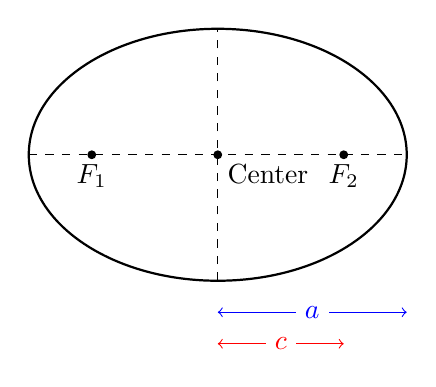
\begin{tikzpicture}[scale=0.8]
      % Draw the ellipse
      \draw[thick] (0,0) ellipse (3cm and 2cm);
      
      % Draw major and minor axes
      \draw[dashed] (-3,0) -- (3,0);
      \draw[dashed] (0,-2) -- (0,2);
      
      % Mark the center
      \fill (0,0) circle (2pt) node[below right] {Center};
      
      % Mark the foci
      \fill (-2,0) circle (2pt) node[below] {$F_1$};
      \fill (2,0) circle (2pt) node[below] {$F_2$};
      
      % Indicate the semi-major axis (a)
      \draw[<->, blue] (0, -2.5) -- (3, -2.5) node[midway, fill=white] {$a$};
      
      % Indicate the focal distance (c)
      \draw[<->, red] (0, -3.0) -- (2, -3.0) node[midway, fill=white] {$c$};
  \end{tikzpicture}
  \end{center}
  Additionally, the semi-minor axis $b$ is related to $a$ and $c$ by:
  
  \bigskip
  \textbf{Key Points:}
  \begin{itemize}
      \item If $e = 0$, the ellipse is a circle.
      \item If $0 < e < 1$, the ellipse is elongated, with greater elongation as $e$ increases.
  \end{itemize}
\end{frame}

\begin{frame}
  \frametitle{Hyperbola}
\begin{block}{Definition}
  The graph of the equation of the form 
  \[
\frac{y^2}{b^2} - \frac{x^2}{a^2} = 1
\]
where \(a,b\) are non-zero numbers
\end{block}
\end{frame}

\begin{frame}
  \begin{figure}
    \centering 
    \includegraphics[scale=0.5]{hyperbola2.png}
  \end{figure}
\end{frame}
\begin{frame}
  \frametitle{Hyperbola}
  \begin{block}{Foci}
    The foci of a hyperbola are two points with the property that the difference of
the distances from the foci to a point on the hyperbola is a constant independent
of the point on the hyperbola
  \end{block}
\end{frame}

\begin{frame}
  \begin{figure}
    \centering 
    \includegraphics[scale=0.4]{hyperbola3.png}
  \end{figure}
\end{frame}
\begin{frame}
  \begin{figure}
    \centering 
    \includegraphics[scale=0.5]{hyperbola1.png}
  \end{figure}
\end{frame}

\subsection{Exponents}
\begin{frame}
  \frametitle{Positive Integer Exponent}
  \begin{block}{Positive Integer Exponent}
    If \(x\) is a real number and \(m\) is a positive integer, then \(x^{m}\) is defined to be the
product with \(x\) appearing \(m\) times
\[x^{m} = \underset{x \;\;appears\;\;m \;\;times}{\underbrace{x \cdot x \cdots x }}\]
    
  \end{block}
\end{frame}

\begin{frame}
  \frametitle{Positive Integer Exponenets}
  \begin{block}{Properties}
    Suppose \(x\) and \(y\) are numbers and \(m\) and \(n\) are positive integers. Then 
    \[x^{m}x^{n} = x^{m+n} \]   
    \[\left(x^{m}\right)^{n} = x^{mn} \] 
    \[x^{m}y^{m} = \left(xy\right)^{m} \] 
  \end{block}
\end{frame}
\begin{frame}
  \frametitle{\(x^{0}\)} 
  \begin{alertblock}{What is \(x^{0}\)}
    If  \(x^{m}x^{n} = x^{m+n}\) then we can write \[x^{0}x^{n} = x^{0+n} = x^{n} \implies x^{0} = 1\;for\;\ x \neq 0\]
   \end{alertblock}

   \begin{alertblock}{What is \(0^{0}\)}
    \begin{itemize}
      \item The rule \( x^0 = 1 \) (for \( x \neq 0 \)) suggests that \( 0^0 \) should be \(1\).
      \item The rule \( 0^m = 0 \) (for \( m > 0 \)) suggests that \( 0^0 \) should be \(0\)
      \item Since these two rules contradict each other, \( 0^0 \) is left undefined in general mathematics.
      \item However, in combinatorics and programming, \( 0^0 \) is often defined as \(1\) for convenience.
  \end{itemize}
   \end{alertblock}
\end{frame}

\begin{frame}
  \frametitle{Negative Integer Exponents}
  If \(x^{m}x^{n} = x^{m+n}\), if we take \(m = -n \), then 
  \[x^{m}x^{-m} = x^{0} = 1 \implies x^{m}x^{-m} = 1\]
  We have to define \(x^{-m}\) to equal the multiplicative inverse of \(x^{m}\)
\begin{block}{Negative Interger Exponent}
  If \(x \neq 0\) and \(m\) is a positive integer, then \(x^{-m}\) is defined to multiplicative inverse of \(x^{m}\) 
  \[x^{-m} = \frac{1}{x^{m}}\]
  
\end{block}
\end{frame}

\begin{frame}
    \frametitle{Exponents: Some Graphs}
    \begin{columns}
      \begin{column}{0.5\textwidth}
        \begin{figure}
          \includegraphics[scale=0.4]{exponent-graph1.png}
          \caption{graph of \(\frac{1}{x}\)}
        \end{figure}
      \end{column}
      \begin{column}{0.5\textwidth}
        \begin{figure}
          \includegraphics[scale=0.4]{exponent-graph2.png}
          \caption{graph of \(\frac{1}{x^{2}}\)}
        \end{figure}
      \end{column}
    \end{columns}
\end{frame}
\begin{frame}
  \frametitle{Negative Integer Exponenets}
  \begin{alertblock}{Graph of Negative Integer Exponents}
    if \(m\) is  a positive integer then
    \begin{itemize}
      \item \(\frac{1}{x^{m}}\) behaves like \(\frac{1}{x}\) if \(m\) is odd
      \item \(\frac{1}{x^{m}}\) behaves like \(\frac{1}{x^{2}}\) if \(m\) is even
      \item Larger values of \(m\) correspond to functions whose graphs get closer to the x-axis more rapidly for large values of \(x\)
      and closer to the vertical axis more rapidly for values of \(x\) near 0
    \end{itemize} 
  \end{alertblock}  

\end{frame}

  \begin{frame}
    \frametitle{Roots}
    \begin{block}{\(m^{th}\) root}
   If \(m\) is a positive integer and \(x\) is a real number, then \(x^{1/m}\) is defined to be the real number satisfying the equation
   \[\left(x^{1/m}\right)^{m} = x \]
  subject to the following conditions:
  \begin{itemize}
    \item  If \(x < 0\) and \(m\) is an even integer, then \(x^{1/m} \)is undefined 
    \item If \(x > 0\) and \(m\) is an even integer, then \(x^{1/m} \) is chosen to be the \textit{\textcolor{red}{positive number}} satisfying the equation above
  \end{itemize}
The number \(x^{1/m}\) is called the \textbf{\(m^{th}\)} root of \(x\).
\end{block}
  
\end{frame}
\begin{frame}
  \frametitle{Roots}
  \begin{example}
    \begin{itemize}
      \item \(8^{1/3}\) and \(-8^{1/3}\)
      \item \(9^{1/2}\) and \(-9^{1/2}\)
    \end{itemize}
  \end{example}
  \begin{solution}
    \begin{enumerate}
      \item \( \left(8^{1/3}\right)^{3} = 8 \implies 2 \)
      \item \( \left(-8^{1/3}\right)^{3} = -8 \implies -2 \). There is no other number other than \(-2\)
      \item \( \left( 9^{1/2} \right)^{2} = -3 \; or \;3\). But as per the rule, we have to choose positive possibility, that is \(3\)
      \item \( \left( -9^{1/2} \right)^{2} \). No number real number exists so no solution 
    \end{enumerate}
  \end{solution}
\end{frame}


\begin{frame}{Rational Exponents}
  \begin{block}{Definition}
  Suppose \(\frac{n}{m}\) is a fraction in reduced form, where \(n\) and \(m\) are integers and \(m > 0\). Then, whenever it makes sense,
  \[
    x^{\frac{n}{m}} = \Bigl(x^{\frac{1}{m}}\Bigr)^n.
  \]
  \vspace{0.5em}
  \textbf{Note:} For the expression \(x^{\frac{1}{m}}\) to be defined, additional conditions on \(x\) may be required (for example, if \(m\) is even, then typically \(x \ge 0\)).
  \end{block}
\end{frame}

\begin{frame}{Algebra of Exponents}
  \begin{block}{Exponent Rules}
    Let \(p, q\) be rational numbers and \(x, y\) be positive numbers. Then the following rules hold:
    \begin{itemize}
      \item \(x^p \cdot x^q = x^{\,p+q}\)
      \item \(x^p \cdot y^p = (xy)^p\)
      \item \((x^p)^q = x^{\,pq}\)
      \item \(x^0 = 1\)
      \item \(x^{-p} = \dfrac{1}{x^p}\)
      \item \(\dfrac{x^p}{x^q} = x^{\,p-q}\)
      \item \(\left(\dfrac{x}{y}\right)^p = \dfrac{x^p}{y^p}\)
    \end{itemize}
  \end{block}
\end{frame}
\subsection{Polynomials}
\begin{frame}{Polynomial Definition}
  \begin{block}{Definition of a Polynomial}
    A polynomial is a function \( p \) such that
    \[
      p(x) = a_0 + a_1 x + a_2 x^2 + \cdots + a_n x^n,
    \]
    where \( n \) is a nonnegative integer and \( a_0, a_1, a_2, \dots, a_n \) are numbers.
  \end{block}
\end{frame}

\begin{frame}{Degree of a Polynomial}
  \begin{block}{Definition}
    Suppose \( p \) is a polynomial defined by
    \[
      p(x) = a_0 + a_1 x + a_2 x^2 + \cdots + a_n x^n.
    \]
    If \( a_n \neq 0 \), then we say that \( p \) has degree \( n \). The degree of \( p \) is denoted by \(\deg p\).
  \end{block}
\end{frame}


\begin{frame}{Polynomial Graphs}
  \centering
  % First Column
  \begin{minipage}[t]{0.45\textwidth}
    \centering
    \includegraphics[width=0.9\linewidth]{polynomial_degree_0.png}\\[1mm]
    \includegraphics[width=0.9\linewidth]{polynomial_degree_1.png}\\[1mm]
  \end{minipage}
  \begin{minipage}[t]{0.45\textwidth}
    \centering
    \includegraphics[width=0.9\linewidth]{polynomial_degree_2.png}
  \end{minipage}
\end{frame}


\begin{frame}
  \centering
  \begin{minipage}[t]{0.45\textwidth}
    \centering
    \includegraphics[width=\linewidth]{polynomial_degree_4.png}\\[1mm]
    \includegraphics[width=\linewidth]{polynomial_degree_7.png}
  \end{minipage}
\end{frame}


\begin{frame}{The Algebra of Polynomials}
  Two functions can be added, subtracted, or multiplied, producing another function. Specifically, if \(p\) and \(q\) are functions, then the functions 
  \[
    p+q,\quad p-q,\quad \text{and} \quad pq
  \]
  are defined by
  \[
    (p+q)(x) = p(x) + q(x),
  \]
  \[
    (p-q)(x) = p(x) - q(x),
  \]
  \[
    (pq)(x) = p(x) \, q(x).
  \]
\end{frame}


\begin{frame}{Degree of the Sum and Difference of Two Polynomials}
  \begin{alertblock}{Important Result}
  If \(p\) and \(q\) are nonzero polynomials, then
  \[
  \deg(p+q) \leq \max\{\deg p,\, \deg q\},
  \]
  and
  \[
  \deg(p-q) \leq \max\{\deg p,\, \deg q\}.
  \]
  \end{alertblock}

 
  \begin{alertblock}{Degree of the Product of Two Polynomials}
    If \(p\) and \(q\) are nonzero polynomials, then
    \[
    \deg(pq) = \deg p + \deg q.
    \]
  \end{alertblock}
\end{frame}


\begin{frame}{Example: Polynomials \(p\) and \(q\)}
  \begin{exampleblock}{Problem}
  Suppose \(p\) and \(q\) are polynomials defined by
  \[
  p(x) = 2 - 3x^2 \quad \text{and} \quad q(x) = 4x + 7x^5.
  \]
  Answer the following:
  \begin{enumerate}
      \item What is \(\deg p\)?
      \item What is \(\deg q\)?
      \item Find a formula for \(pq\).
      \item What is \(\deg(pq)\)?
  \end{enumerate}
  \end{exampleblock}
\end{frame} 
\begin{frame}
  \begin{exampleblock}{Solution}
  \begin{enumerate}
      \item Since \(p(x) = 2 - 3x^2\) has the highest power \(x^2\), we have \(\deg p = 2\).
      \item For \(q(x) = 4x + 7x^5\), the highest power is \(x^5\), so \(\deg q = 5\).
      \item The product \(pq\) is computed as follows:
      \[
      pq = (2-3x^2)(4x+7x^5) = 2\cdot 4x + 2\cdot 7x^5 - 3x^2\cdot 4x - 3x^2\cdot 7x^5,
      \]
      which simplifies to:
      \[
      pq = 8x - 12x^3 + 14x^5 - 21x^7.
      \]
      \item The highest power in \(pq\) is \(x^7\), so \(\deg(pq) = 7\).
  \end{enumerate}
  \end{exampleblock}
  \end{frame}


  \begin{frame}{Zeros/Roots of a Function}
    \begin{block}{Definition}
      A number \(t\) is called a zero of a function \(p\) if
      \[
        p(t) = 0.
      \]
    \end{block}
  \end{frame}

  \begin{frame}{Closed-Form Expression}
    \begin{block}{Definition}
      A closed-form expression is an explicit formula that can be written using a finite number of standard operations and functions (e.g., addition, multiplication, exponentiation, logarithms, trigonometric functions). It does not involve infinite series, integrals, or iterative processes.
    \end{block}
    \vspace{0.5em}
    \textbf{Example:} The quadratic formula,
    \[
      x = \frac{-b \pm \sqrt{b^2-4ac}}{2a},
    \]
    is a closed-form expression.
  \end{frame}
  
  \begin{frame}{Zeros of Higher–Degree Polynomials}
    \begin{block}{Key Points}
      \begin{itemize}
        \item The quadratic formula gives exact zeros for degree–2 polynomials.
        \item Although formulas exist for cubics and quartics, they are rarely used.
        \item No closed-form formula exists for polynomials of degree 5 or higher.
        \item Numerical methods can approximate zeros for any polynomial.
        \item \textbf{Example:} For 
        \[
          p(x)=x^5-5x^4-6x^3+17x^2+4x-7,
        \]
        approximate zeros are:
        \[
          -1.80,\; -0.73,\; 0.63,\; 1.48,\; 5.56.
        \]
      \end{itemize}
    \end{block}
  \end{frame}

\begin{frame}
  \frametitle{Zeros on graph}
  \centering
  \includegraphics[scale=0.23]{zeros.png}

\end{frame}

\begin{frame}
  \frametitle{Zeros on graph}
  \begin{columns}
    \begin{column}{0.5\textwidth}
      \centering
      \includegraphics[scale=0.3]{no-real-zeros.png}
    \end{column}
    \begin{column}{0.5\textwidth}
      The function \(x^{2}+1\) has no real zeros 
    \end{column}
  \end{columns}
\end{frame}

\begin{frame}{Factor of a Polynomial}
  \begin{block}{Definition}
    Suppose \(p\) is a polynomial and \(t\) is a real number. Then \(x-t\) is called a \emph{factor} of \(p(x)\) if there exists a polynomial \(G(x)\) such that
    \[
      p(x) = (x-t)\,G(x)
    \]
    for every real number \(x\).
  \end{block}
\end{frame}

\begin{frame}{Example: Factors and Zeros of a Polynomial}
  \begin{exampleblock}{Problem}
    Let 
    \[
      p(x) = (x-2)(x-5)(x^2+1).
    \]
    \begin{enumerate}[(a)]
      \item Explain why \(x-2\) is a factor of \(p(x)\).
      \item Explain why \(x-5\) is a factor of \(p(x)\).
      \item Show that \(2\) and \(5\) are zeros of \(p\).
      \item Show that \(p\) has no (real) zeros except \(2\) and \(5\).
    \end{enumerate}
  \end{exampleblock}
\end{frame}
\begin{frame}
  \begin{block}{Solution}
    \begin{enumerate}[(a)]
      \item The polynomial is given in factored form as \((x-2)(x-5)(x^2+1)\). Since \((x-2)\) appears as one of the factors, it is a factor of \(p(x)\).
      \item Similarly, \((x-5)\) appears explicitly in the factorization, so it is a factor of \(p(x)\).
      \item To show that \(2\) and \(5\) are zeros, substitute:
        \[
          p(2) = (2-2)(2-5)(2^2+1) = 0\cdot(-3)\cdot5 = 0,
        \]
        \[
          p(5) = (5-2)(5-5)(5^2+1) = 3\cdot0\cdot26 = 0.
        \]
        Thus, \(p(2)=0\) and \(p(5)=0\).
      \item The factor \(x^2+1\) yields \(x^2=-1\), which has no real solutions. Hence, aside from the zeros from \((x-2)\) and \((x-5)\), there are no other real zeros.
    \end{enumerate}
  \end{block}
\end{frame}

\begin{frame}{Zeros and Factors of a Polynomial}
  \begin{block}{Key Fact}
    Suppose \(p\) is a polynomial and \(t\) is a real number. Then \(t\) is a zero of \(p\) if and only if \(x-t\) is a factor of \(p(x)\).
  \end{block}
\end{frame}

\begin{frame}{Number of Zeros of a Polynomial}
  \begin{block}{Fundamental Property}
    A nonzero polynomial \(p(x)\) of degree \(n\) has at most \(n\) zeros.
  \end{block}

  \begin{block}{Explanation}
    A polynomial of degree 15 has at most 15 zeros. This is because each (real) zero \(t_j\) of a polynomial \(p\) corresponds to a factor \((x-t_j)\) in a factorization of the form
    \[
      p(x) = (x-t_1)(x-t_2)\cdots(x-t_m) \, G(x),
    \]
    where \(G(x)\) is a polynomial with no (real) zeros. If \(p(x)\) had more than 15 zeros, then the right-hand side would represent a polynomial of degree higher than 15, contradicting the fact that \(p\) is of degree 15.
  \end{block}
\end{frame}


\begin{frame}{Behavior of a Polynomial Near \(\pm\infty\)}
  \begin{block}{Key Concepts}
    \begin{itemize}
      \item \textbf{\(x\) near \(+\infty\):} \(x\) is very large.
      \item \textbf{\(x\) near \(-\infty\):} \(x\) is very negative (i.e., \(|x|\) is very large).
      \item Our goal is to determine whether a polynomial \(p(x)\) is positive or negative in these extremes.
    \end{itemize}
  \end{block}
\end{frame}

\begin{frame}
  \centering
  \includegraphics[scale=0.2]{at-infty.png}

%  \centering
%  \includegraphics[scale=0.2]{at-infty2.png}

\end{frame}
 

\begin{frame}{Behavior of a Polynomial Near \(\pm\infty\)}
  \begin{block}{Key Ideas}
    \begin{itemize}
      \item To analyze the behavior as \(x\to\pm\infty\), factor out the highest degree term.
      \item If \(c\,x^n\) is the highest degree term in \(p(x)\), then for very large \(|x|\), \(p(x)\) behaves like \(c\,x^n\).
    \end{itemize}
  \end{block}
\end{frame}
   

\begin{frame}{Zero in an Interval}
  \begin{block}{Intermediate Value Theorem}
    Suppose \(p\) is a polynomial and \(a, b \in \mathbb{R}\) with \(a < b\). If \(p(a)\) and \(p(b)\) have opposite signs, then there exists a number \(c \in (a, b)\) such that \(p(c)=0\).
  \end{block}
\end{frame}


\begin{frame}{Example 7: Zero in an Interval}
  \begin{exampleblock}{Problem}
    Let 
    \[
      p(x) = x^5 + x^2 - 1.
    \]
    Explain why \(p\) has a zero in the interval \((0,1)\).
  \end{exampleblock}
  
  \begin{block}{Solution}
    Evaluate the polynomial at the endpoints:
    \[
      p(0) = 0^5 + 0^2 - 1 = -1 \quad \text{and} \quad p(1) = 1^5 + 1^2 - 1 = 1.
    \]
    Since \(p(0) < 0\) and \(p(1) > 0\), by the Intermediate Value Theorem, there exists a \(c \in (0,1)\) such that \(p(c)=0\).
  \end{block}
\end{frame}

\begin{frame}{Zeros for Polynomials with Odd Degree}
  \begin{block}{Key Result}
    Every polynomial with odd degree has at least one real zero.
  \end{block}
  \vspace{0.5em}
  \begin{itemize}
    \item For a polynomial \(p(x)\) of odd degree, as \(x \to -\infty\), \(p(x)\) tends to \(-\infty\) (or \(+\infty\)) and as \(x \to \infty\), \(p(x)\) tends to \(+\infty\) (or \(-\infty\)).
    \item By the Intermediate Value Theorem, since \(p(x)\) changes sign, there exists at least one real number \(c\) such that \(p(c)=0\).
  \end{itemize}
\end{frame}

\begin{frame}{Graph of \(p(x)=x^4-4x^3-2x^2+13x+12\)}
  % \centering
  % \includegraphics[width=\textwidth]{polynomial_plots.pdf}
\end{frame}

\begin{frame}{Choosing an Appropriate Graphing Interval}
  \begin{block}{Key Concepts}
    \begin{itemize}
      \item When graphing a polynomial, choose an interval that displays its peaks, valleys, and asymptotic behavior.
      \item For the polynomial
      \[
        p(x)=x^4-4x^3-2x^2+13x+12,
      \]
      an interval that is too narrow (e.g., \([-2,2]\)) fails to show its behavior as \(|x|\) grows.
      \item An interval like \([-2,4]\) better reveals the local extrema (peaks/valleys) and the fact that for large \(|x|\), \(p(x)\) behaves like \(x^4\).
      \item Using an excessively large interval (e.g., \([-50,50]\)) may hide the local features due to scaling.
      \item \textbf{Conclusion:} The interval \([-2,4]\) provides a good balance to illustrate the key features of the graph.
    \end{itemize}
  \end{block}
\end{frame}

\subsection{Rational Function}
\begin{frame}{Rational Function}
  \begin{block}{Definition}
    A \emph{rational function} is a function \(r\) defined by
    \[
      r(x) = \frac{p(x)}{q(x)},
    \]
    where \(p(x)\) and \(q(x)\) are polynomials, with \(q(x) \neq 0\).
  \end{block}
\end{frame}

\begin{frame}{Domain of a Rational Function \& Example for \(r(x)\)}
  \begin{block}{General Rule}
    The domain of a rational function 
    \[
      \frac{p(x)}{q(x)}
    \]
    is the set of all real numbers where the expression makes sense. Since division by 0 is undefined, we exclude all zeros of \(q(x)\).
  \end{block}
\end{frame}

\begin{frame}
  \begin{exampleblock}{Example }
    \[r(x)=\frac{3x^5+x^4-6x^3-2}{x^2-9}\]
    Factor the denominator:
    \[
      x^2-9=(x-3)(x+3).
    \]
    Thus, \(r(x)\) is undefined at \(x=3\) and \(x=-3\). Hence, its domain is
    \[
      \{x\in\mathbb{R}: x\neq 3 \text{ and } x\neq -3\}.
    \]
  \end{exampleblock}
\end{frame}

\begin{frame}{}
  \begin{exampleblock}{Example}
    \[s(x)=\frac{x^3-6x+5}{x^4+9}\]
    The denominator \(x^4+9\) is always positive (since \(x^4\ge 0\) and \(9>0\)). Therefore, \(s(x)\) is defined for every real number. \\
    Domain of \(s(x)\) :
    \(
      \mathbb{R}
    \)
  \end{exampleblock}
\end{frame}

\begin{frame}{Advantages of Mixed Representation}
  \begin{block}{Mixed Representation}
    Expressing a rational function as a polynomial plus a proper rational function (one where the numerator's degree is less than the denominator's) is analogous to writing an improper fraction as an integer plus a proper fraction.
  \end{block}
  \vspace{0.5em}
  \begin{block}{Advantages}
    \begin{itemize}
      \item \textbf{Simplification:} It makes further operations (such as integration, differentiation, and partial fraction decomposition) easier.
      \item \textbf{Asymptotic Insight:} The polynomial part reveals the behavior of the function as \(x\to\pm\infty\), while the proper fraction (the remainder) tends to zero for large \(|x|\).
      \item \textbf{Clarity:} It separates the "whole" part from the "fractional" part, making the function's structure more transparent.
    \end{itemize}
  \end{block}
\end{frame}

\begin{frame}{Mixed Rational Function Representation}
  \begin{exampleblock}{Problem}
    Express
    \[
      \frac{x^5 + 6x^3 + 11x + 7}{x^2+4}
    \]
    in the form
    \[
      G(x) + \frac{ax+b}{x^2+4},
    \]
    where \(G(x)\) is a polynomial and \(a, b\) are constants.
  \end{exampleblock}
\end{frame}

\begin{frame}{Procedure for Dividing Polynomials}
  \begin{block}{Steps}
    \begin{enumerate}
      \item \textbf{Rewrite:} Express the highest-degree term in the numerator as a single term times the denominator, plus the necessary adjustment.
      \item \textbf{Simplify:} Use the rewritten numerator to simplify the quotient.
      \item \textbf{Iterate:} Repeat steps (1) and (2) on the remaining rational function until the degree of the numerator is less than the degree of the denominator or the numerator becomes 0.
    \end{enumerate}
  \end{block}
\end{frame}

\begin{frame}{Mixed Representation Example (Part 1)}
  \begin{exampleblock}{Problem}
    Express
    \[
      \frac{x^5+6x^3+11x+7}{x^2+4}
    \]
    in the form
    \[
      G(x)+\frac{ax+b}{x^2+4},
    \]
    where \(G(x)\) is a polynomial and \(a, b\) are constants.
  \end{exampleblock}
\end{frame}
\begin{frame}
  \begin{block}{Step 1: Eliminate the \(x^5\) Term}
    Notice that
    \[
      x^5=x^3(x^2+4)-4x^3.
    \]
    Therefore,
    \[
    \begin{aligned}
      x^5+6x^3 &= x^3(x^2+4)-4x^3+6x^3\\[1mm]
               &= x^3(x^2+4)+2x^3.
    \end{aligned}
    \]
    So we can write:
    \[
      \frac{x^5+6x^3+11x+7}{x^2+4}=x^3+\frac{2x^3+11x+7}{x^2+4}.
    \]
  \end{block}
\end{frame}

\begin{frame}{Mixed Representation Example (Part 2)}
  \begin{block}{Step 2: Eliminate the \(2x^3\) Term}
    Write
    \[
      2x^3=2x(x^2+4)-8x.
    \]
    Then,
    \[
    \begin{aligned}
      2x^3+11x+7 &= 2x(x^2+4)-8x+11x+7\\[1mm]
                  &= 2x(x^2+4)+(3x+7).
    \end{aligned}
    \]
    Thus,
    \[
      \frac{2x^3+11x+7}{x^2+4}=2x+\frac{3x+7}{x^2+4}.
    \]
  \end{block}
\end{frame} 
\begin{frame}
  \begin{block}{Final Mixed Representation}
    Combining the steps, we have:
    \[
      \frac{x^5+6x^3+11x+7}{x^2+4}=x^3+2x+\frac{3x+7}{x^2+4}.
    \]
  \end{block}
\end{frame}

\begin{frame}{Division Algorithm for Polynomials}
  \begin{block}{General Result}
    If \(p(x)\) and \(q(x)\) are polynomials with \(q(x) \neq 0\), then there exist unique polynomials \(G(x)\) and \(R(x)\) such that
    \[
      \frac{p(x)}{q(x)} = G(x) + \frac{R(x)}{q(x)},
    \]
    where either \(R(x)=0\) or \(\deg R < \deg q\). Equivalently, we can write
    \[
      p(x)=q(x)G(x)+R(x).
    \]
  \end{block}
\end{frame}


\begin{frame}{Division by \(x-t\) and Zeros of a Polynomial}
  \begin{block}{Special Case}
    Fix a real number \(t\) and let \(q(x)=x-t\). Since \(\deg q=1\), the remainder \(R(x)\) is a constant \(c\)(Because degree \(R < \)degree \(q\)). Thus, there exist a polynomial \(G(x)\) and a constant \(c\) such that
    \[
      p(x) = (x-t)G(x) + c.
    \]
    Evaluating at \(x=t\) yields \(p(t)=c\), so we can rewrite this as
    \[
      p(x) = (x-t)G(x) + p(t).
    \]
  \end{block}
  \vspace{0.5em}
  \begin{block}{Application to Zeros}
    \(t\) is a zero of \(p\) if and only if \(p(t)=0\), which happens precisely when
    \[
      p(x)=(x-t)G(x).
    \]
  \end{block}
\end{frame}

\begin{frame}{Behavior of a Rational Function Near \(\pm\infty\)}
  \begin{block}{General Approach}
    To determine the behavior of a rational function as \(x\to\pm\infty\), factor out the highest power of \(x\) in the numerator and the denominator.
  \end{block}
\end{frame} 
\begin{frame}
  \begin{block}{Example}
    Consider 
    \[
      r(x)=\frac{9x^5-2x^3+1}{x^8+x+1}.
    \]
    The highest degree in the numerator is \(x^5\) and in the denominator is \(x^8\). Factoring these out yields:
    \[
      r(x) \sim \frac{9x^5}{x^8}=\frac{9}{x^3}.
    \]
    As \(|x|\) becomes very large:
    \begin{itemize}
      \item \(r(x)\to 0\) as \(x\to\infty\) (approaching \(0^+\)).
      \item \(r(x)\to 0\) as \(x\to-\infty\) (approaching \(0^-\)).
    \end{itemize}
  \end{block}
\end{frame}

\begin{frame}{Asymptote of a Rational Function}
  \begin{block}{Definition}
    A line is an asymptote of a graph if the graph becomes and stays arbitrarily close to the line as \(x\) tends to \(\pm\infty\).
  \end{block}
  \vspace{0.5em}
  \begin{exampleblock}{Finding the Asymptote}
    Consider
    \[
      r(x)=\frac{3x^6-9x^4+6}{2x^6+4x+3}.
    \]
    Both the numerator and the denominator are degree 6. Therefore, the horizontal asymptote is the ratio of the leading coefficients:
    \[
      y=\frac{3}{2}.
    \]
  \end{exampleblock}
\end{frame}
\begin{frame}
  \begin{figure}
    \centering
    \includegraphics[scale=0.2]{asymptote1.png}
  \end{figure}
\end{frame}

\begin{frame}{Asymptote}
  \begin{exampleblock}{Example}
    \[
      r(x) = \frac{4x^{10}-2x^3+3x+15}{2x^6+x^5+1}
    \]
  \end{exampleblock}
  \begin{block}{Solution}
    \[
      \frac{4x^{10}}{2x^6} = 2x^4.
    \]
    Thus, as \(|x|\to\infty\), \(r(x)\) behaves like \(x^{4}\). That is, \(r(x)\) is very large and positive when \( x \to \infty\) and \( x \to -\infty\) 
  \end{block}
\end{frame}


\end{document}